\documentclass[a4paper]{book}

\usepackage[]{fullpage}
\usepackage[portuguese]{babel}
\usepackage{graphicx}
\usepackage{hyperref}
\usepackage{natbib}
\usepackage[export]{adjustbox}

\usepackage{lipsum}

\title{Hello Git\\
\large Um tutorial para usar o Git imediatamente}
\author{Francisco de Assis Boldt}
\date{\today}
  
\begin{document}
  
\maketitle
  
\tableofcontents

\chapter{O hello world do Git}

Este tutorial apresenta uma forma muito simples de se usar o Git.
Como exemplo, serão feitas algumas versões do clássico programa, 
``hello world''. Essas versões serão gerenciadas pelo sistema 
controlador de versões Git.
A intenção é mostrar uma forma de se começar a usar Git em 
dentro de poucos minutos. É apenas um primeiro contato com a ferramenta.
Nenhum conteúdo é abordado por completo ou com profundidade.
Para isso, são sugeridas obras como \cite{hodson2014ry} e 
\cite{chacon2014pro}.
Mesmo assim, é bom deixar claro que Git é um sistema de
gerenciamento de versões de software.
Porém, apesar de ter sido idealizado para o desenvolvimento
de programas, também pode ser usado para outras finalidades
como escrita compartilhada de textos ou edição de imagens.
O Git mantém um histórico das alterações de um repositório 
permitindo recuperar informações, dividir as tarefas em ramos
e mesclar alterações que podem ser feitas independentemente.

\section{Iniciando um repositório}

Fisicamente no computador, um repositório Git é apenas um
diretório com algumas metainformações sobre as alterações 
dos arquivos do projeto que está no diretório.
A figura \ref{fig:01} mostra como criar um repositório Git
do zero. O comando \texttt{mkdir greetings} cria o diretório
onde colocaremos o código do nosso projeto de exemplo e o
comando \texttt{cd greetings}  acessa o diretório criado.
Pode-se ver pelo comando \texttt{ls -a} que ainda não existe
nenhum  arquivo no diretório. Para transformar esse diretório
vazio em um repositório Git basta executar o comando
\texttt{git init}, que o repositório será iniciado, conforme
mostra a repetição do comando \texttt{ls -a}.

\begin{figure}[ht]
\caption{Criando um repositório}
\label{fig:01}
\centering
\includegraphics[scale=0.6,left]{"images/01-Criando um repositório.png"}
\end{figure}

Note que foi criado um diretório oculto (por que começa com
um ponto (.)), e por isso só é listado (\texttt{ls}) quando
se usa o parâmetro \texttt{-a}. A árvore com todos os arquivos
e subdiretórios criado pelo comando \texttt{git init} pode ser
vista na figura \ref{fig:02}. O comando \texttt{tree .git} foi
usado para exibir essa árvore. O diretório \texttt{.git} contém
metadados. Ou seja, é um diretório com dados para o Git
controlar os dados do repositórios. É a forma do Git
``lembrar'' da história do projeto.
Um repositório Git nada mais é do que um diretório com um
subdiretório \texttt{.git} adequadamente estruturado.
O subdiretório \texttt{.git} não deve ser alterado diretamente.
Suas alterações devem ser feitas através do comando
\texttt{git} acompanhado dos parâmetros correspondentes à ação
desejada.

\begin{figure}[ht]
\caption{Árvore de diretórios do repositório}
\label{fig:02}
\centering
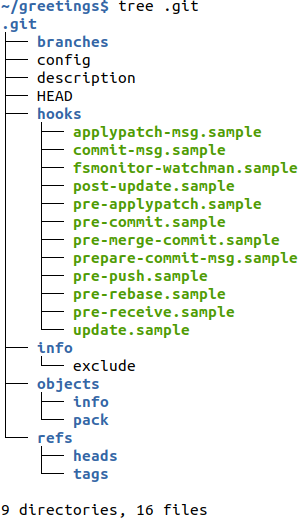
\includegraphics[scale=0.6,left]{"images/02-Árvore de diretórios do repositório.png"}
\end{figure}

\section{O comando \texttt{git status}}

Um comando que é usado o tempo todo em um repositório Git é o comando
\texttt{git status} apresentado na figura \ref{fig:03}.
Apesar desse comando estar em uma seção dedicada a ele, 
devido a sua importância, ele não será abordado em profundidade,
uma vez que nosso objetivo aqui é mostrar uma utilização do Git
com poucos comandos, sem explorá-los por completo.

\begin{figure}[ht]
\caption{Status de um repositório recém criado}
\label{fig:03}
\centering
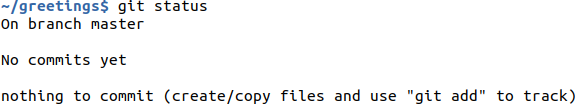
\includegraphics[scale=0.6,left]{"images/03-Status de um repositório recém criado.png"}
\end{figure}

A primeira linha de resposta é \texttt{On branch master}.
\textit{Banches} são ramificações de um projeto Git, 
que podem tomar rumos diferentes durante seu desenvolvimento.
Diferentes ramos podem ser mesclados ou se tornarem novos projetos.
O nome \texttt{master} é o nome padrão para o ramo inicial do projeto Git.
Particularmente, eu nunca vi um projeto Git sem o ramo master,
mas não existe nenhuma exigência de que esse ramo exista.
É que normalmente não se muda esse nome.
%
A segunda linha é \texttt{No commits yet}.
Os \textit{commits} são fotografias do sistema que o Git mantém
em seus metadados no diretório \texttt{.git}.
Como não fizemos nenhum \textit{commit} ainda, não existe nenhuma
``fotografia'' no Git.
%
A terceira linha é 
\texttt{nothing to commit (creat/copy files and use "git add" to track)}.
Não há nada para ``fotografar'' (\textit{commit}) por que o diretório
do projeto está vazio.
Nenhum arquivo está sendo monitorado.
Para monitorar um arquivo temos que usar o comando \texttt{git add},
que é apresentado na pŕoxima seção.


\section{Criando e monitorando um arquivo}

Como pode ser traduzido da terceira linha de resposta da figura
\ref{fig:03}, o Git monitora (\textit{track}) arquivos criados
ou copiados para dentro do diretório do repositório.
A figura \ref{fig:04} mostra o conteúdo que queremos no arquivo
\texttt{greet.py}.
Este arquivo em texto simples pode ser criado dentro do diretório
ou copiado para dentro dele.
É um arquivo escrito em linguagem de programação Python 3.
Porém, não é necessário saber Python para acompanhar este tutorial.
Basta notar que o arquivo será alterado e cada alteração será monitorada
pelo Git. A execução do arquivo com o comando \texttt{python greed.py} é 
opcional. O comando \texttt{ls -a} é só para mostrar que o arquivo 
\texttt{greed.py} foi criado.

\begin{figure}[ht]
\caption{Criando o primeiro arquivo do projeto}
\label{fig:04}
\centering
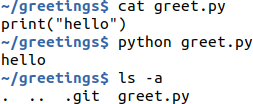
\includegraphics[scale=0.6,left]{"images/04-Criando o primeiro arquivo do projeto.png"}
\end{figure}

Depois de criado o arquivo \texttt{greet.py}, o comando
\texttt{git status} mostrará uma resposta um pouco diferente,
como mostra a figura figura \ref{fig:05}.
As duas primeiras linhas de resposta continuam iguais,
mais agora, a terceira linha de resposta lista o arquivo
\texttt{greet.py} em vermelho, e diz que ele não está
sendo monitorado (\textit{untracked}).
Veja que a resposta do comando já diz como adicionar
a modificação no monitoramento (\texttt{git add <file>}).
Aqui é um ponto que merece uma atenção especial quando se usa o Git.
O Git só ``fotografa'' (\textit{commit}) as alterações que estão
em uma área abstrata de sua organização chamada \textit{stage}.
Isso por que, muitas vezes fazemos alterações que não queremos 
gravar. Testamos algo, não gostamos do resultado, e queremos descartar
o que foi feito. Outras vezes, queremos gravar só algumas alterações,
mas não todas. 
Esse processo também nos permite fazer alterações variadas e 
agrupá-las em fotografias separadas.

\begin{figure}[ht]
\caption{Status com arquivo fora da área de stage}
\label{fig:05}
\centering
\includegraphics[scale=0.6,left]{"images/05-Status com arquivo fora da área de stage.png"}
\end{figure}

A figura \ref{fig:06} mostra como adicionar um arquivo na área de 
\textit{stage} do Git, com o comando \texttt{git add greet.py}.
Note que agora o arquivo está listado em verde, mas ainda não foi
``fotografado'' (\textit{committed}).
Se você colocar um arquivo na área de \textit{stage} por engano,
pode removê-lo de lá, sem excluí-lo do diretório, com o 
comando \texttt{git rm --cached <file>}, como mostra a resposta 
do comando \texttt{git status}.

\begin{figure}[ht]
\caption{Status com arquivo na da área de stage}
\label{fig:06}
\centering
\includegraphics[scale=0.6,left]{"images/06-Status com arquivo na da área de stage.png"}
\end{figure}

É importante resaltar que até o momento, nenhum arquivo está
sendo monitorado pelo Git.
O arquivo \texttt{greet.py} está pronto para ser ``fotografado'' e,
a partir daí, ser monitorado.
Para fotografar as mudanças que estão na área de \textit{stage}
deve-se executar o comando da figura \ref{fig:07}.
Entretanto, o comando só será aceito se você estiver com 
seu nome e email configurado.
Para não entrar em detalhes de configuração agora, 
você pode digitar os comandos 
\texttt{git config user.name `SEU\_PRIMEIRO\_NOME SEU\_ULTIMO\_NOME'} e
\texttt{git config user.email `SEU\_EMAIL@example.com'}.
Quando se executa o comando \texttt{git commit} sem o parâmetro
\texttt{-m `comentário'}, o Git abre um editor de texto para que 
um comentário sobre a fotografia seja escrito.
O Git não permite commits sem comentários.
Então, foi usado aqui o \texttt{-m} para ficar mais resumido e 
visível através das figuras.

\begin{figure}[ht]
\caption{Primeira fotografia do repositório}
\label{fig:07}
\centering
\includegraphics[scale=0.6,left]{"images/07-Primeira fotografia do repositório.png"}
\end{figure}

Se você quiser ver a fotografia tirada do sistema
você pode usar o comando \texttt{git show} e terá um resultado
parecido com o da figura \ref{fig:08}.
Vamos entender essa fotografia, mas sem seguir a ordem em que 
os dados aparecem.
Vemos o comentário inserido pelo comando \texttt{git commit}.
Também vemos a data e hora de quando o commit foi executado,
que pode ser entendida como o momento da fotografia.
A linha que começa com \texttt{Author} tem os dados inseridos
pelos comandos \texttt{git config <etc>}.
Em negrito, está indicado que essa é uma fotografia que
contém um arquivo novo, e a linha verde que começa com +
é o conteúdo do arquivo.

\begin{figure}[ht]
\caption{Vendo detalhes da fotografia mais recente do sistema}
\label{fig:08}
\centering
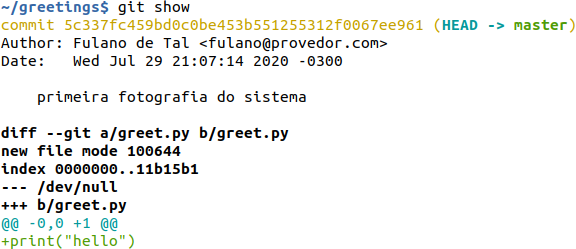
\includegraphics[scale=0.6,left]{"images/08-Vendo detalhes da fotografia mais recente do sistema.png"}
\end{figure}

Na primeira linha, em amarelo, logo depois da palavra commit,
está o \textit{hash} da fotografia.
O \textit{hash} é a assinatura, o identificador, da fotografia.
Podemos usar esse identificador para acessar a fotografia
posteriormente. Na mesma linha, em negrito e verde, temos a
palavra \textbf{master},
indicando que o ramo do projeto chamado \textbf{master} está
apontando para esta fotografia no momento.
Ainda na mesma linha, em azul, temos a palavra \textbf{HEAD} 
seguida
dos sinais de $-$ e $>$ representando uma seta (\texttt{->}).
Esta seta indica que o estado do sistema que estamos vendo no
momento está apontando para o ramos master.
Isso ficará mais claro a seguir.

\chapter{Criando fotografias novas e acessando fotografias antigas}

O Git só vai tirar uma nova fotografia do sistema se algo for 
alterado e colocado na área de stage.
A figura \ref{fig:09} mostra a alteração sugerida.
O resultado do programa continuou quase igual, por isso
a palavra ``hello'' foi colocada toda em maiúsculo 
para ficar mais clara que uma alteração foi feita.

\begin{figure}[ht]
\caption{Fazendo uma alteração}
\label{fig:09}
\centering
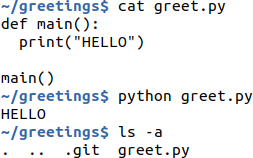
\includegraphics[scale=0.6,left]{"images/09-Fazendo uma alteração.png"}
\end{figure}

Depois da alteração do arquivo, o comando \texttt{git status}
apresenta um retorno diferente, como mostra a figura 
\ref{fig:10}.
Novamente o arquivo \texttt{greet.py} está em vermelho
por não estar na área de stage,
mas agora esse arquivo está sendo monitorado. 
Então temos duas opções.
Podemos descartar as alterações com o comando 
\texttt{git restore greet.py} ou podemos adicionar 
as alterações na área de stage com o comando
\texttt{git add greet.py}.
Adicionaremos as alterações na área de stage, como mostra a
figura \ref{fig:11}.

\begin{figure}[ht]
\caption{Status com arquivo modificado fora da area de stage}
\label{fig:10}
\centering
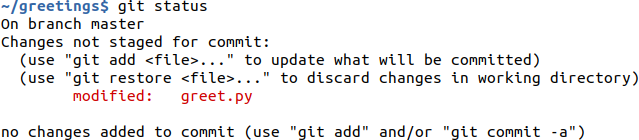
\includegraphics[scale=0.6,left]{"images/10-Status com arquivo modificado fora da area de stage.png"}
\end{figure}


\begin{figure}[ht]
\caption{Status com arquivo modificado na da area de stage}
\label{fig:11}
\centering
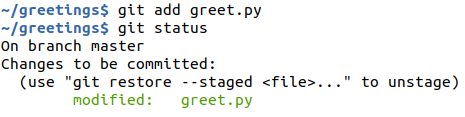
\includegraphics[scale=0.6,left]{"images/11-Status com arquivo modificado na da area de stage.png"}
\end{figure}

O resultado do comando \texttt{git status} está muito parecido 
com o da figura \ref{fig:06}. Agora, em verde, não aparece
mais ``arquivo novo'' (new file), mas ``modificado'' (modified).
%
A figura \ref{fig:12} mostra o comando \texttt{git commit} com o
parâmetro \texttt{-m} e um comentário relacionado à alteração feita.
O comando \texttt{git show} mostra como ficou a fotografia.
A linha em vermelho que inicia com o sinal $-$ mostra
o que foi removido, e as linhas em verde que iniciam com
o sinal $+$ mostram o que foi adicionado.

\begin{figure}[ht]
\caption{Atualizando o repositório e vendo os detalhes da atualização}
\label{fig:12}
\centering
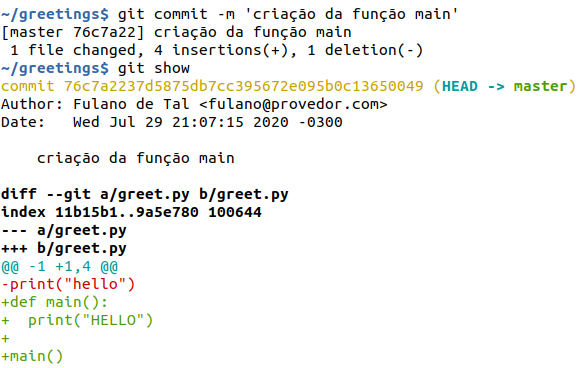
\includegraphics[scale=0.6,left]{"images/12-Atualizando o repositório e vendo os detalhes da atualização.png"}
\end{figure}

Vamos fazer mais uma alteração no sistema, que pode ser
vista na figura \ref{fig:13}.
Novamente, o resultado do programa é virtualmente o mesmo,
e para que a alteração seja um pouco mais evidente, 
a palavra \textit{Hello} foi colocada agora apenas com
a primeira letra em maiúsculo.

\begin{figure}[ht]
\caption{Fazendo mais uma alteração}
\label{fig:13}
\centering
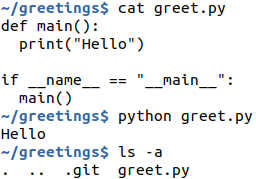
\includegraphics[scale=0.6,left]{"images/13-Fazendo mais uma alteração.png"}
\end{figure}

Depois dessa alteração, o comando \texttt{git status}
apresentará o mesmo retorno visto na figura \ref{fig:10}.
Vamos adicionar à área de stage a nova alteração com
o comando \texttt{git add greet.py}.
Após executado esse comando, o status do repositório
será igual ao apresentado na figura \ref{fig:11}.
%
Agora estamos prontos para executar o comando \texttt{commit} 
como mostra a figura \ref{fig:14}.
Novamente podem ser vistas as alterações feitas observando-se
as linhas verdes e vermelhas.

\begin{figure}[ht]
\caption{Atualizando com a terceira alteração}
\label{fig:14}
\centering
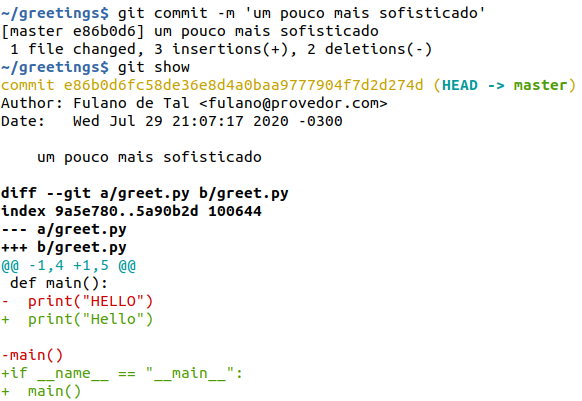
\includegraphics[scale=0.6,left]{"images/14-Atualizando com a terceira alteração.png"}
\end{figure}

Agora temos cópias seguras das versões anteriores
do nosso projeto. 

\newpage
\section{Listando as fotografias do repositório}

A figura \ref{fig:15} mostra como listar as fotografias do 
sistema com o comando \texttt{git log}.
A opção \texttt{--oneline} foi usada aqui para que 
as fotografias sejam vistas de um forma mais compacta.
Mas vocë deve testar sem essa opção também.
%
\begin{figure}[ht]
\caption{Listando as fotografias do repositório}
\label{fig:15}
\centering
\includegraphics[scale=0.6,left]{"images/15-Listando as fotografias do repositório.png"}
\end{figure}

As fotografias do repositório são apresentadas em ordem cronológica
reversa. Ou seja, a última fotografia é a primeira a ser apresentada
e a primeira fotografia é a última.
Em amarelo vemos o hash de cada fotografia.
Normalmente, essa parte do hash é suficiente para acessar a
fotografia.
Por exemplo, é possível ver uma fotografia mais antiga 
(ou mais recente) com o comando \texttt{git show <hash>},
onde normalmente a parte do hash que aparece na figura
\ref{fig:15} é suficiente para identificá-la.

\newpage
\section{Mostrando o conteúdo de fotografias}

Na figura \ref{fig:16} o comando \texttt{git show}
mostra a fotografia anterior usando apenas a parte de seu hash
listada na figura \ref{fig:15}.

\begin{figure}[ht]
\caption{Vendo detalhes da fotografia anterior}
\label{fig:16}
\centering
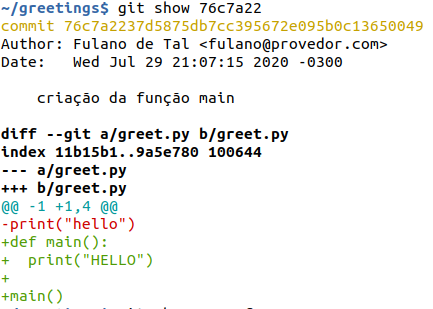
\includegraphics[scale=0.6,left]{"images/16-Vendo detalhes da fotografia anterior.png"}
\end{figure}

A figura \ref{fig:17} mostra a primeira fotografia do repositório.

\begin{figure}[ht]
\caption{Vendo detalhes da fotografia da primeira fotografia}
\label{fig:17}
\centering
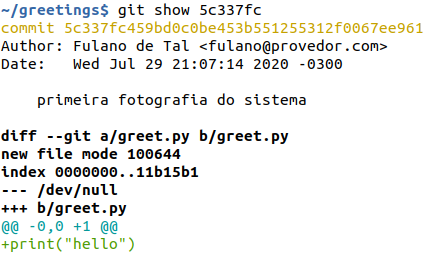
\includegraphics[scale=0.6,left]{"images/17-Vendo detalhes da fotografia da primeira fotografia.png"}
\end{figure}

\newpage
\section{Alterando o estado do sistema}

O comando \texttt{git checkout} permite colocar o repositório
em um estado gravado em alguma fotografia. 
A figura \ref{fig:18} mostra como fazer o repositório
voltar para o estado em que a função \texttt{main}
foi criada.

\begin{figure}[ht]
\caption{Voltando o sistema para o estado da fotografia anterior}
\label{fig:18}
\centering
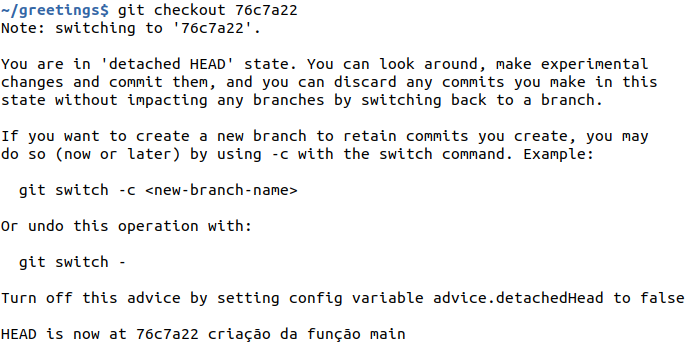
\includegraphics[scale=0.6,left]{"images/18-Voltando o sistema para o estado da fotografia anterior.png"}
\end{figure}

Veja na figura \ref{fig:20} que o programa \texttt{greet.py}
voltou ao seu estado anterior.

\begin{figure}[ht]
\caption{Estados dos arquivos do sistema depois de voltar uma fotografia}
\label{fig:20}
\centering
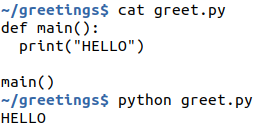
\includegraphics[scale=0.6,left]{"images/20-Estados dos arquivos do sistema depois de voltar uma fotografia.png"}
\end{figure}

Ao listar as fotografias do repositório, como mostra a figura 
\ref{fig:19}, o comando \texttt{git log} não mostra mais o brach master, nem a fotografia da última alteração feita.
Além disso, \textbf{HEAD} agora está na fotografia da segunda 
alteração.

\begin{figure}[ht]
\caption{Listando fotografias tão ou mais antigas que a atual}
\label{fig:19}
\centering
\includegraphics[scale=0.6,left]{"images/19-Listando tão ou mais antigas que a atual.png"}
\end{figure}

Você pode estar se perguntando ``Git é então um complexo ctrl+z?''. Claro que não!
A fotografia mais recente continua sendo monitorada e 
pode ser visualizada com a opção \texttt{--all}
no comando \texttt{git log}, como mostra a 
figura \ref{fig:21}.

\begin{figure}[!h]
\caption{Listando todas fotografias do repositório}
\label{fig:21}
\centering
\includegraphics[scale=0.6,left]{"images/21-Listando todas fotografias do repositório.png"}
\end{figure}

%Na verdade, o Git sempre adiciona informação ao repositório.
%Mesmo sendo possível remover informações de um repositório,
%isso é raramente recomendado.

A figura \ref{fig:22} mostra como colocar o sistema no
estado da fotografia mais recente.

\begin{figure}[ht]
\caption{Voltando para versão mais recente do sistema}
\label{fig:22}
\centering
\includegraphics[scale=0.6,left]{"images/22-Voltando para versão mais recente do sistema.png"}
\end{figure}

Observe que \textbf{HEAD} não está mais apontando para 
\textbf{master}. \textbf{HEAD} sempre estará no estado 
atual do repositório. Mas isso não significa que o estado 
atual é o mais recente.

\section{Criando etiquetas para fotografias}

Para facilitar o acesso das fotografias pode-se etiquetá-las.
O tipo de etiqueta mais comum é mostrado na figura
\ref{fig:23}, que usa o comando \texttt{git tag} com a
opção \texttt{-a}. Esta opção permite usar a opção 
\texttt{-m} para inserir um comentário na etiqueta.

\begin{figure}[ht]
\caption{Criando etiquetas para a fotografia atual}
\label{fig:23}
\centering
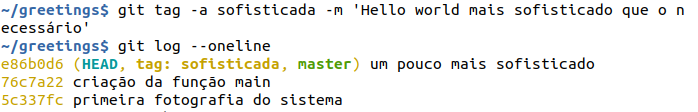
\includegraphics[scale=0.6,left]{"images/23-Criando etiquetas para a fotografia atual.png"}
\end{figure}

O comando \texttt{git tag} coloca a etiqueta na fotografia atual
do sistema, mas é possível etiquetar outras fotografias 
através de seu hash, como mostra a figura \ref{fig:25}.

\begin{figure}[!h]
\caption{Etiquetando uma fotografia mais antiga}
\label{fig:25}
\centering
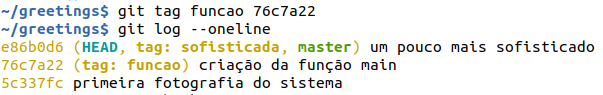
\includegraphics[scale=0.6,left]{"images/25-Etiquetando uma fotografia mais antiga.png"}
\end{figure}

A figura \ref{fig:26} mostra coma acessar uma fotografia antiga 
através de sua etiqueta

\begin{figure}[!h]
\caption{Acessando uma fotografia antiga através da sua etiqueta}
\label{fig:26}
\centering
\includegraphics[scale=0.6,left]{"images/26-Acessando uma fotografia antiga através da sua etiqueta.png"}
\end{figure}

O comando \texttt{git tag} pode ser usado para listar as
etiqueta, como mostra a figura \ref{fig:28}.

\begin{figure}[!h]
\caption{Listando todas as etiquetas do repositório}
\label{fig:28}
\centering
\includegraphics[scale=0.6,left]{"images/28-Listando todas as etiquetas do repositório.png"}
\end{figure}

%Listagens mais complexas, com caracteres coringa por exemplo, 
%podem ser feitas com esse comando, mas não serão exploradas aqui.

Quando se executa o comando \texttt{git show} com uma etiqueta,
ele mostra também os dados da etiqueta, como pode ser visto na
figura \ref{fig:24}.
A informação de quem fez a etiqueta (tagger) e de quando 
a etiqueta foi criada só é gravada se a opção \texttt{-a}
for usada na criação dela.

\begin{figure}[!h]
\caption{Mostrando fotografias usando etiquetas}
\label{fig:24}
\centering
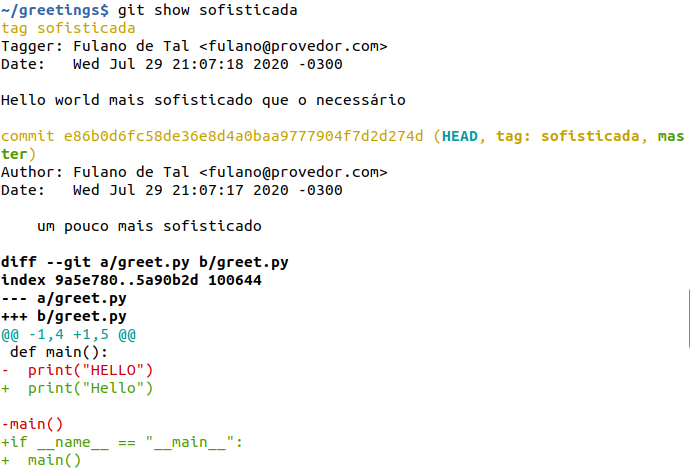
\includegraphics[scale=0.6,left]{"images/24-Mostrando fotografias usando etiquetas.png"}
\end{figure}


Para acessar a fotografia mais recente podemos usar o 
comando mostrada na figura \ref{fig:27}.

\begin{figure}[ht]
\caption{Acessando a fotografia mais recente através da sua etiqueta}
\label{fig:27}
\centering
\includegraphics[scale=0.6,left]{"images/27-Acessando a fotografia mais recente através da sua etiqueta.png"}
\end{figure}

É importante notar que \textbf{HEAD} não aponta para nenhum
branch. No caso, não aponta para \textbf{master}, que é 
o único branch do repositório.
Para continuar o tutorial execute o comando da
figura \ref{fig:29}, para que \textbf{HEAD} aponte para 
\textbf{master}.

\begin{figure}[ht]
\caption{Acessando o branch master}
\label{fig:29}
\centering
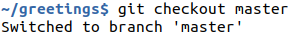
\includegraphics[scale=0.6,left]{"images/29-Acessando o branch master.png"}
\end{figure}

Visto que este é um tutorial superficial, não será explicado o motivo deste procedimento.

\chapter{Ramos no projeto}

As etiquetas são fixadas em uma fotografia, mas ramos
(braches) são vivos e acompanham novas fotografias que 
são criadas.
Há muitas formas de se usar os braches.
Neste capítulo mostraremos uma delas.
Também há vários motivos para se usar os branches.
Um deles é que você pode inserir uma alteração instável
no sistema e querer que essa alteração fique gravada.
Ou seja, você fez uma alteração que não está pronta,
mas quer que essa alteração seja monitorada pelo Git por
algum motivo.
Talvez você não tenha certeza que o próximo passo vai funcionar,
ou talvez você queira testar o próximo passo de mais do que uma
forma. Ou ainda, pode ser que outra pessoa termine essa 
atualização parcial que você fez.
O fato é que você não quer que esta seja a versão usada até 
que ela esteja terminada.

\section{Criando ramos}

Como ilustração, faremos uma versão brasileira para o nosso
programa. Como eu supostamente ainda não sei se isso será
fácil ou difícil de terminar, farei um branch como mostra a
figura \ref{fig:30}.
Agora a fotografia mais recente tem dois ramos (na cor verde),
\textbf{master} e \textbf{pt-br}.

\begin{figure}[ht]
\caption{Criando um novo branch}
\label{fig:30}
\centering
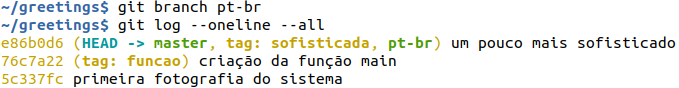
\includegraphics[scale=0.6,left]{"images/30-Criando um novo branch.png"}
\end{figure}

Para fazer um alteração no ramo \textbf{pt-br}, deve-se mudar 
\textbf{HEAD} para esse ramo, como apresentado na figura
\ref{fig:31}. Agora \textbf{HEAD} aponta para \textbf{pt-br}.

\begin{figure}[ht]
\caption{Acessando um branch}
\label{fig:31}
\centering
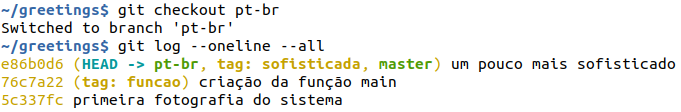
\includegraphics[scale=0.6,left]{"images/31-Acessando um branch.png"}
\end{figure}

Quando só existia o ramo \textbf{master}, cada comando
\texttt{commit} movia o ramo \textbf{master} para a
fotografia mais recente.
Agora que \textbf{HEAD} aponta para \textbf{pt-br},
o comando \texttt{commit} vai mover o ramo \textbf{pt-br}
para as novas fotografias, deixando o ramo
\textbf{master} na fotografia atual.
Assim, fica claro para todos os envolvidos no projeto
que o ramo \textbf{master} contém uma versão estável
do sistema.

\section{Uma alteração incompleta para o ramos atual}

Como ilustração será feita a alteração proposta na
figura \ref{fig:32}.

\begin{figure}[ht]
\caption{Alterando o sistema no branch atual}
\label{fig:32}
\centering
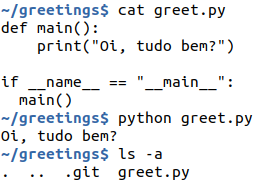
\includegraphics[scale=0.6,left]{"images/32-Alterando o sistema no branch atual.png"}
\end{figure}

A resposta do comando \texttt{git status} da figura
\ref{fig:33} já é conhecida. 
A única diferença do que já foi visto é a primeira linha
que mostra que ramo atual é o \textbf{pt-br} 
(\textit{On branch pt-br}).

\begin{figure}[ht]
\caption{Status do novo branch com arquivo modificado fora da área de stage}
\label{fig:33}
\centering
\includegraphics[scale=0.6,left]{"images/33-Status do novo branch com arquivo modificado fora da área de stage.png"}
\end{figure}

O status após adicionar a alteração na área de stage
mostrado na figura \ref{fig:34} também não é muito 
diferente do que já foi visto.

\begin{figure}[ht]
\caption{Status do novo branch com arquivo modificado na da área de stage}
\label{fig:34}
\centering
\includegraphics[scale=0.6,left]{"images/34-Status do novo branch com arquivo modificado na da área de stage.png"}
\end{figure}

O resultado dos comandos \texttt{git commit} 
e \texttt{git show} apresentados na
figura \ref{fig:35} também não apresentam muita novidade.

\begin{figure}[!h]
\caption{Fotografia da versão brasileira do sistema}
\label{fig:35}
\centering
\includegraphics[scale=0.6,left]{"images/35-Fotografia da versão brasileira do sistema.png"}
\end{figure}

Note que o ramo \textbf{master} não tem nada de especial.
Usar outro nome para um ramo não muda nada no processo
de fotografar as versões do sistema.

\newpage
\section{Terminado a alteração desejada}

Para mostrar como colocar uma alteração no ramo estável do
sistema, vamos fazer a alteração proposta na 
figura \ref{fig:36}.
Estamos considerando o ramo estável deste repositório
o ramo \textbf{master}, mas poderia ser qualquer outro nome.

\begin{figure}[ht]
\caption{Parametrizando o sistema}
\label{fig:36}
\centering
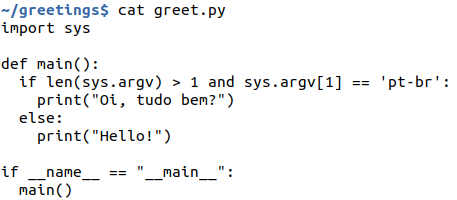
\includegraphics[scale=0.6,left]{"images/36-Parametrizando o sistema.png"}
\end{figure}

Depois de colocar a nova alteração na área de stage
e executar o comando \texttt{commit} podemos ver a nova 
fotografia listada na figura \ref{fig:38}.

\begin{figure}[ht]
\caption{Lista das fotografias após a versão brasileira parametrizada}
\label{fig:38}
\centering
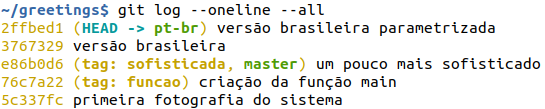
\includegraphics[scale=0.6,left]{"images/38-Lista das fotografias após a versão brasileira parametrizada.png"}
\end{figure}

A figura \ref{fig:37} mostra como ficou a fotografia
mais recente do repositório.
Também mostra como executar o programa na versão
mais recente, caso ache interessante.

\begin{figure}[ht]
\caption{Fotografia da versão brasileira atualizada}
\label{fig:37}
\centering
\includegraphics[scale=0.6,left]{"images/37-Fotografia da versão brasileira atualizada.png"}
\end{figure}

\section{Mesclando o ramo atual com o ramo principal}

Agora que a alteração já foi finalizada, é hora de 
mesclar a atualização no ramo principal.
A figura \ref{fig:39} apresenta um procedimento que pode
ser executado com essa finalidade.
Primeiro, temos que fazer \textbf{HEAD} apontar
para o ramo principal com o comando 
\texttt{git checkout master}.
Depois, usamos o comando \texttt{git merge pt-br}
para mesclar o ramo \textbf{pt-br} com o ramo atual.

\begin{figure}[ht]
\caption{Mesclando a versão brasileira com a versão original}
\label{fig:39}
\centering
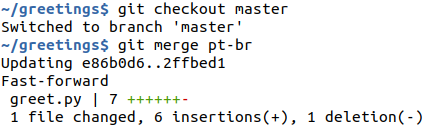
\includegraphics[scale=0.6,left]{"images/39-Mesclando a versão brasileira com a versão original.png"}
\end{figure}

A figura \ref{fig:40} mostra a lista de fotografias
depois da mesclagem de ramos.

\begin{figure}[ht]
\caption{Listando as fotografias do repositório após mesclar versões do sistema}
\label{fig:40}
\centering
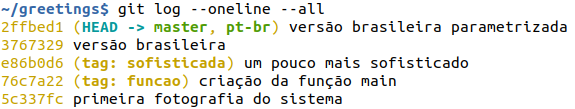
\includegraphics[scale=0.6,left]{"images/40-Listando as fotografias do repositório após mesclar versões do sistema.png"}
\end{figure}

Na segunda linha da reposta do comando
\texttt{git merge pt-br} na figura \ref{fig:39} 
está escrito \textit{Fast-forward}.
Isso significa que nenhuma alteração foi feita no
ramo \textbf{master} enquanto o ramo \textbf{pt-br}
estava sendo alterado.
Assim, não houve nenhum conflito para juntar as versões
porque a versão mais recente de \textbf{pt-br}
era como uma versão futura de \textbf{master}.
A seguir, veremos um situação que isso não é resolvido tão
facilmente.

\chapter{Criando bifurcações no projeto}

O capítulo anterior mostrou uma mesclagem do tipo
\textit{fast-forward}, que é um tipo sem conflito.
Aqui, veremos como resolver conflitos quando ele acontecem.

\section{Criando um ramo comum}

Agora faremos uma versão do sistema em alemão.
Para manter uma boa prática de Git vamos criar um novo
ramo, como mostra a figura \ref{fig:41}.

\begin{figure}[ht]
\caption{Criando um branch para uma versão em alemão}
\label{fig:41}
\centering
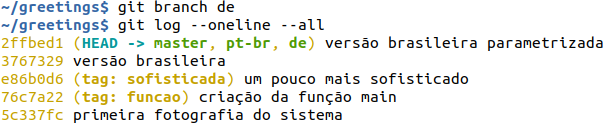
\includegraphics[scale=0.6,left]{"images/41-Criando um branch para uma versão em alemão.png"}
\end{figure}

Para trabalhar no novo ramo, deve-se usar o comando
\texttt{git checkout}. O comando \texttt{git log}
mostra o ramo para o qual \textbf{HEAD} aponta.
O resoltado pode ser visto na figura \ref{fig:42}.

\begin{figure}[ht]
\caption{Acessando o branch onde será implementada a versão alemã do sistema}
\label{fig:42}
\centering
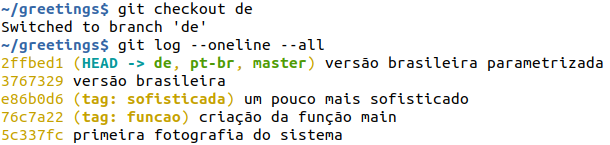
\includegraphics[scale=0.6,left]{"images/42-Acessando o branch onde será implementada a versão alemã do sistema.png"}
\end{figure}

Depois de fazer a alteração sugerida na figura \ref{fig:43},
execute o comando \texttt{git commit} para deixar 
gravada as alterações no repositório.

\begin{figure}[ht]
\caption{Alteração feita para versão alemã do sistema}
\label{fig:43}
\centering
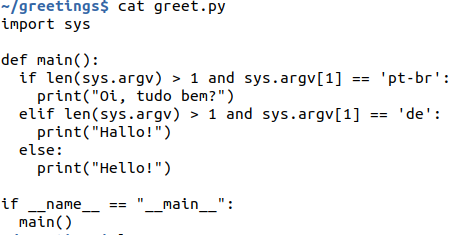
\includegraphics[scale=0.6,left]{"images/43-Alteração feita para versão alemã do sistema.png"}
\end{figure}

A fotografia do último \textit{commit} está na figura
\ref{fig:44}.

\begin{figure}[ht]
\caption{Fotografando a versão alemã do sistema}
\label{fig:44}
\centering
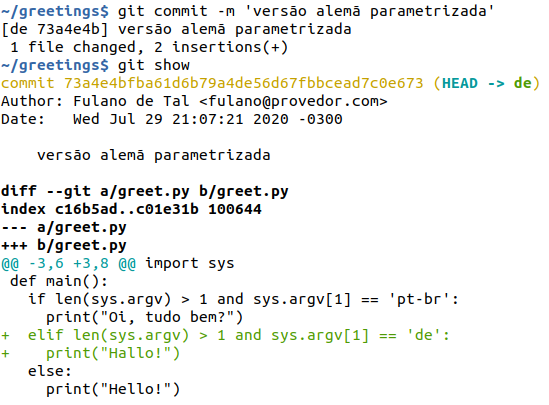
\includegraphics[scale=0.6,left]{"images/44-Fotografando a versão alemã do sistema.png"}
\end{figure}

A figura \ref{fig:45} mostra que o sistema possui seis 
fotografias até o momento.

\begin{figure}[!h]
\caption{Listando as fotografias após a inclusão da versão alemã}
\label{fig:45}
\centering
\includegraphics[scale=0.6,left]{"images/45-Listando as fotografias após a inclusão da versão alemã.png"}
\end{figure}

Na condição atual, no exemplo co capítulo anterior,
o ramo foi mesclado com o ramo estável.
Mas para exemplificar um conflito, não vamos mesclá-lo 
agora.
Um motivo para não mesclar é não ter feito todos os
testes no seu ramo.
Ou o ramo ainda não está terminado.
Vamos supor me nossa situações hipotética que 
não temos certeza que a resposta correta em alemão
é \textit{hallo}.
Por isso, vamos adiar a mesclagem com o ramo principal.

\newpage
\section{Criando mais um ramo comum}

Normalmente, conflitos de mesclagem não são criados 
intencionalemente. Mas para ilustrar a resolução 
de conflitos que inevitavelmente acontecerão,
vamos fazer uma versão em italiano do nosso 
sistema para forçar um conflito.
Para isso, vamos começar criando um novo ramo a
partir de \textbf{master}.
Após fotografarmos a alteração do sistema
com a versão italiana, teremos dois ramos que
nasceram a partir de \textbf{master}.
Um deles é facilmente mesclável. O outro, nem tanto.

Uma forma de se criar um ramo a partir de \textbf{master}
é estando com \textbf{HEAD} apontando para \textbf{master}.
Em seguida, usa-se o comando \texttt{git branch} para 
criar um novo branch, como na figura \ref{fig:46}.

\begin{figure}[ht]
\caption{Criando um branch para implementar uma versão italiana a partir da versão brasileira}
\label{fig:46}
\centering
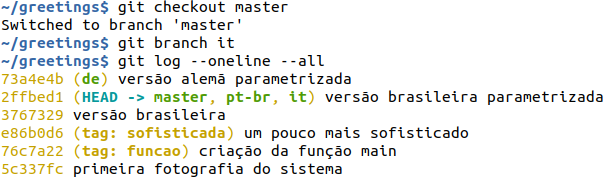
\includegraphics[scale=0.6,left]{"images/46-Criando um branch para implementar uma versão italiana a partir da versão brasileira.png"}
\end{figure}

Note que \textbf{HEAD} continua apontando para
\textbf{master}.
Portanto é necessário mover \textbf{HEAD} para o novo
ramo, como figura \ref{fig:47}.

\begin{figure}[ht]
\caption{Acessando o branch da versão italiana}
\label{fig:47}
\centering
\includegraphics[scale=0.6,left]{"images/47-Acessando o branch da versão italiana.png"}
\end{figure}

Implemente a alteração sugerida na figura \ref{fig:48}.

\begin{figure}[ht]
\caption{Implementando a versão italiana}
\label{fig:48}
\centering
\includegraphics[scale=0.6,left]{"images/48-Implementando a versão italiana.png"}
\end{figure}

Adicione as alterações na área de stage e execute
o comando \texttt{git commit} para fazer a nova fotografia.

%Após adicionar as alterações na área de stage e executar
%o comando \texttt{git commit} a fotografia mais atual
%deverá estar parecida com a da figura \ref{fig:49}.
%
%\begin{figure}[ht]
%\caption{Visualizando a fotografia da versão italiana}
%\label{fig:49}
%\centering
%\includegraphics[scale=0.6,left]{"images/49-Visualizando a fotografia da versão italiana.png"}
%\end{figure}

\newpage
\section{Listando as fotografias em forma de grafo}

A opção \texttt{--graph} do comando \texttt{git log}
lista as fotografias do repositório em forma de grafo,
como na figura \ref{fig:50}.


\begin{figure}[!h]
\caption{Listando todas as fotografias do repositório em forma de grafo}
\label{fig:50}
\centering
\includegraphics[scale=0.6,left]{"images/50-Listando todas as fotografias do repositório em forma de grafo.png"}
\end{figure}

Note que acima do ramo \textbf{master} as linhas estão
vermelhas, indicando um possível conflito.
Observe que o ramo \textbf{de} (alemão), que é mais
antigo que o ramo \textbf{it} (italiano), se mostra como
um ramo que está saindo de um galho.



\section{Mesclando o último ramo antes do primeiro}

O último ramo criado foi o ramo \textbf{it},
mas aqui vasmos mesclá-lo ao ramo principal
antes do ramo mais antigo, que é o ramo \textbf{de}.
A figura \ref{fig:51} mostra uma forma de como isso 
pode ser feito.
Ocorreu uma mesclagem do tipo \textit{fast-forward}
sem nenhum problema.

\begin{figure}[ht]
\caption{Mesclando a versão italiana com a principal}
\label{fig:51}
\centering
\includegraphics[scale=0.6,left]{"images/51-Mesclando a versão italiana com a principal.png"}
\end{figure}

Na figura \ref{fig:52} podemos ver que o grafo não foi 
alterado, mas agora \textbf{HEAD} e \textbf{master}
estão na fotografia mais recente.

\begin{figure}[!h]
\caption{Listando todas as fotografias do repositório em forma de grafo após mesclar a versão italiana}
\label{fig:52}
\centering
\includegraphics[scale=0.6,left]{"images/52-Listando todas as fotografias do repositório em forma de grafo após mesclar a versão italiana.png"}
\end{figure}

\newpage
\section{Quando não corre tudo bem na mesclagem}

Agora, veja figura \ref{fig:53} o que ocorre quando tentamos 
mesclar o ramo alemão com o ramo princial.

\begin{figure}[ht]
\caption{Mesclando a versão alemã com a principal}
\label{fig:53}
\centering
\includegraphics[scale=0.6,left]{"images/53-Mesclando a versão alemã com a principal.png"}
\end{figure}

O comando \texttt{git mergetool --tool-help}
lista as disponíveis no seu sistema operacional
(figura \ref{fig:54}).

\begin{figure}[!h]
\caption{Buscando ajuda com mergetool}
\label{fig:54}
\centering
\includegraphics[scale=0.6,left]{"images/54-Buscando ajuda com mergetool.png"}
\end{figure}

Conforme a figura \ref{fig:54}, a ferramenta \texttt{vimdiff}
pode ser selecionada como na figura \ref{fig:55}.

\begin{figure}[!h]
\caption{Escolhendo programa para usar com mergetool}
\label{fig:55}
\centering
\includegraphics[scale=0.6,left]{"images/55-Escolhendo programa para usar com mergetool.png"}
\end{figure}

A figura \ref{fig:56} mostra como deve estar o
arquivo \texttt{greet.py} depois de resolvidos os conflitos.
A solução apresentada é apenas uma sugestão da
resolução do conflito que ocorreu.
Outras soluções poderiam ter resolvido o conflito 
também.

\begin{figure}[!ht]
\caption{Programa após a resolução de conflitos}
\label{fig:56}
\centering
\includegraphics[scale=0.6,left]{"images/56-Programa após a resolução de conflitos.png"}
\end{figure}

A utilização do \texttt{vimdiff} excede o escopo deste 
tutorial, mas você pode ver como é a apresentação dessa 
ferramenta na figura \ref{fig:57}.

\begin{figure}[!h]
\caption{vimdiff}
\label{fig:57}
\centering
\includegraphics[scale=0.31]{"images/57-vimdiff.png"}
\end{figure}


Depois de usar uma ferremanta de solução de conflitos
para solucioná-los, o comando \texttt{git commit}
deve ser executado para fotografar a forma como
os conflitos foram solucionados.
%
A figura \ref{fig:58} mostra como os ramos separados 
se juntam depois da solução de conflitos.

\begin{figure}[!h]
\caption{Listando todas as fotografias do repositório em forma de grafo após mesclar a versão alemã}
\label{fig:58}
\centering
\includegraphics[scale=0.5,left]{"images/58-Listando todas as fotografias do repositório em forma de grafo após mesclar a versão alemã.png"}
\end{figure}

Agora, você já sabe uma forma de se usar o Git.
A forma apresentada aqui não é a única, nem a melhor. 
É um exemplo para ser aplicado imediatamente.
É claro que um projeto real, que necessite de um
gerenciador de versões, possívelmente terá mais arquivos
no que o exemplo \texttt{hello world} apresentado aqui.
Porém, trabalhar com mais arquivos pode facilitar o
gerenciamento das versões.
Conflitos geralmente ocorrem quando o mesmo arquivo
sofre alterações em ramos diferentes.


%\chapter{Repositório remoto}

\bibliographystyle{plainnat}
\bibliography{references}

\end{document}

